
\documentclass[11pt,a4paper]{article}

\usepackage[T1]{fontenc}
\usepackage[utf8]{inputenc}
\usepackage[dutch]{babel}
\usepackage{lmodern}
\usepackage{microtype}
\usepackage[a4paper,margin=2.2cm]{geometry}
\usepackage{amsmath,amssymb}
\usepackage{booktabs,array,tabularx}
\usepackage{enumitem}
\usepackage{xcolor}
\usepackage{tikz}
\usetikzlibrary{arrows.meta,decorations.pathmorphing,positioning,calc}

\definecolor{notegray}{RGB}{245,245,245}
\definecolor{uncertain}{RGB}{145,70,0}

\newcommand{\uncertain}[1]{\textcolor{uncertain}{\textit{[onzeker: #1]}}}
\newcommand{\literalnote}[1]{%
  \begin{center}
  \fcolorbox{black!35}{notegray}{%
    \begin{minipage}{0.92\linewidth}
      #1
    \end{minipage}}
  \end{center}
}

\title{\textbf{Kwantum Natuurkunde}\\
\large LaTeX-transcriptie van PDF-pagina's 1--5}
\author{}
\date{}

\begin{document}
\maketitle

\noindent
Deze transcriptie is gebaseerd op visuele inspectie van de scans op hoge resolutie.
De oorspronkelijke spelling en formulering zijn zoveel mogelijk behouden.
Onduidelijke passages zijn gemarkeerd met \uncertain{tekst}.
Schematische tekeningen zijn in TikZ gereconstrueerd en zijn niet bedoeld als
pixel-identieke kopieën.

\section*{PDF-pagina 1 --- omslag}

\begin{center}
\vspace{1.5cm}
{\Huge \textbf{Kwantum}}\\[0.35cm]
{\LARGE \textbf{Natuurkunde}}
\vfill
\uncertain{handtekening of naam onderaan de omslag}
\end{center}

\newpage
\section*{PDF-pagina 2 --- inleiding}

\subsection*{Linker notitiepagina}

\begin{center}
{\LARGE \textbf{Inleiding}}
\end{center}

\literalnote{\centering Alles is in beweging in de natuur.}

\medskip
\noindent
Associatie tussen elementen en platonische lichamen:

\begin{center}
\begin{tabular}{ll}
\toprule
\textbf{Element} & \textbf{Vorm}\\
\midrule
Vuur      & tetra\\
Lucht     & octa\\
Aarde     & hexa\\
Water     & icosa\\
Universum & dodeca\\
\bottomrule
\end{tabular}
\end{center}

\begin{center}
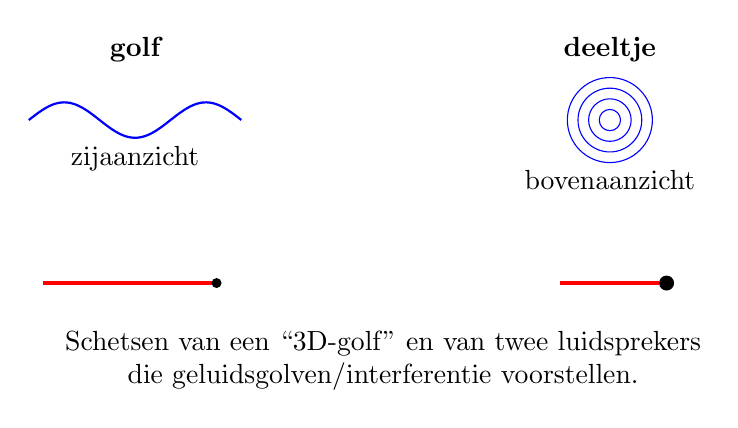
\begin{tikzpicture}[>=Latex,scale=0.9]
  \node[font=\bfseries] at (-3.5,2.2) {golf};
  \node[font=\bfseries] at (3.2,2.2) {deeltje};

  % Golf, zijaanzicht
  \draw[thick,blue,domain=-5:-2,samples=80,smooth]
       plot (\x,{1.2+0.25*sin(180*(\x+5))});
  \node at (-3.5,0.65) {zijaanzicht};

  % Golf, bovenaanzicht
  \foreach \r in {0.15,0.3,0.45,0.6}
    \draw[blue] (3.2,1.2) circle (\r);
  \node at (3.2,0.35) {bovenaanzicht};

  % Deeltje, zijaanzicht
  \draw[very thick,red] (-4.8,-1.1)--(-2.4,-1.1);
  \fill (-2.35,-1.1) circle (2pt);

  % Deeltje, bovenaanzicht
  \draw[very thick,red] (2.5,-1.1)--(3.9,-1.1);
  \fill (4.0,-1.1) circle (3pt);

  \node[align=center] at (0,-2.2)
    {Schetsen van een ``3D-golf'' en van twee luidsprekers\\
     die geluidsgolven/interferentie voorstellen.};
\end{tikzpicture}
\end{center}

\subsection*{Rechter notitiepagina}

\begin{enumerate}[label=\arabic*.,leftmargin=1.8em]
  \item Massa is roterende lading.
  \item Zwaartekracht is ``perfect inklappen van een lading''.
        \uncertain{het woord ``inklappen'' is zwak geschreven}
  \item Licht beweegt voort door een oneindige constructieve
        golfinterferentie.
\end{enumerate}

\literalnote{%
Deze theorie doet me denken aan de gedachtengang van een superintelligent
wezen, \uncertain{``die van ideeën heeft/leeft door moeilijke gedachten''}.}

\begin{align*}
\text{elektromagnetisme} + \text{general relativity}
  &\longrightarrow \text{unified field theory}.
\end{align*}

\newpage
\section*{PDF-pagina 3 --- golven}

\subsection*{Linker notitiepagina}

De genoteerde relaties zijn:

$$
\text{snelheid}=\text{frequentie}\times\text{golflengte}
$$

$$
\text{golflengte}=\frac{\text{snelheid}}{\text{frequentie}}.
$$

In gebruikelijke symbolen:

\begin{align*}
v &= f\lambda,\\
\lambda &= \frac{v}{f}.
\end{align*}

\begin{center}
\begin{tabular}{>{\bfseries}lcc}
\toprule
 & weinig energie & veel energie\\
\midrule
lage frequentie &
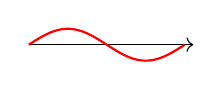
\begin{tikzpicture}[baseline=-0.6ex,x=0.55cm,y=0.45cm]
 \draw[->] (0,0)--(3.8,0);
 \draw[red,thick,domain=0:3.6,samples=60] plot(\x,{0.45*sin(100*\x)});
\end{tikzpicture}
&
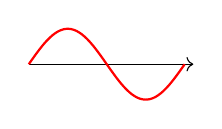
\begin{tikzpicture}[baseline=-0.6ex,x=0.55cm,y=0.45cm]
 \draw[->] (0,0)--(3.8,0);
 \draw[red,thick,domain=0:3.6,samples=60] plot(\x,{1.0*sin(100*\x)});
\end{tikzpicture}
\\[1.2em]
hoge frequentie &
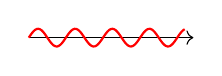
\begin{tikzpicture}[baseline=-0.6ex,x=0.55cm,y=0.45cm]
 \draw[->] (0,0)--(3.8,0);
 \draw[red,thick,domain=0:3.6,samples=100] plot(\x,{0.25*sin(420*\x)});
\end{tikzpicture}
&
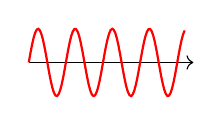
\begin{tikzpicture}[baseline=-0.6ex,x=0.55cm,y=0.45cm]
 \draw[->] (0,0)--(3.8,0);
 \draw[red,thick,domain=0:3.6,samples=100] plot(\x,{0.95*sin(420*\x)});
\end{tikzpicture}
\\
\bottomrule
\end{tabular}
\end{center}

\literalnote{%
Licht is als een dans van magnetisch veld naar elektrisch veld en opnieuw.
De golflengtes zijn de stappen en de frequentie is de beat.}

\subsection*{Rechter notitiepagina: ``Hoe werkt een golf?''}

\begin{description}[style=nextline,leftmargin=3.2cm]
  \item[Frequentie] $f=$ trillingen per seconde.
  \item[Golflengte] $\lambda=$ lengte van één sinus.
  \item[Amplitude] $A=$ hoogte van de trilling.
  \item[Snelheid] $v=$ afstand gedeeld door tijd,
        of frequentie maal golflengte.
\end{description}

\begin{align*}
v &= \frac{\text{afstand}}{\text{tijd}},\\
v &= f\lambda.
\end{align*}

\begin{center}
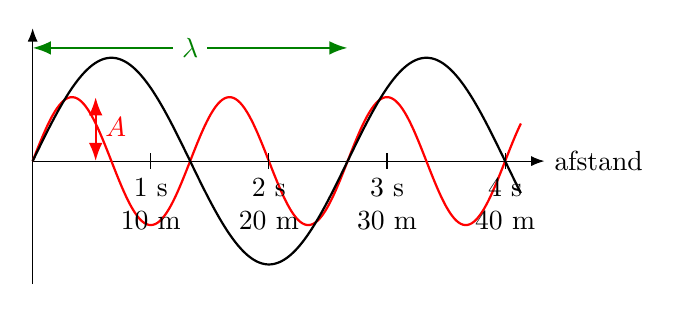
\begin{tikzpicture}[x=0.1cm,y=1.25cm,>=Latex]
  \draw[->] (0,0)--(65,0) node[right] {afstand};
  \draw[->] (0,-1.25)--(0,1.35);
  \draw[thick,red,domain=0:62,samples=220,smooth]
       plot(\x,{0.65*sin(18*\x)});
  \draw[thick,black,domain=0:62,samples=220,smooth]
       plot(\x,{1.05*sin(9*\x)});

  \draw[<->,green!50!black,thick] (0,1.15)--(40,1.15);
  \node[green!50!black,fill=white] at (20,1.15) {$\lambda$};

  \draw[<->,red,thick] (8,0)--(8,0.65);
  \node[red,right] at (8,0.35) {$A$};

  \foreach \x/\lab in {15/{1 s\\10 m},30/{2 s\\20 m},45/{3 s\\30 m},60/{4 s\\40 m}}
    \draw (\x,0.08)--(\x,-0.08) node[below,align=center] {\lab};
\end{tikzpicture}
\end{center}

\newpage
\section*{PDF-pagina 4 --- fotonen, fononen en röntgenstraling}

\subsection*{Linker notitiepagina}

\begin{align*}
\text{foton} &\longrightarrow \text{licht}.
\end{align*}

\literalnote{%
Elektromagnetische golf: elektrische en magnetische componenten
``interlocken'' met elkaar.}

\begin{center}
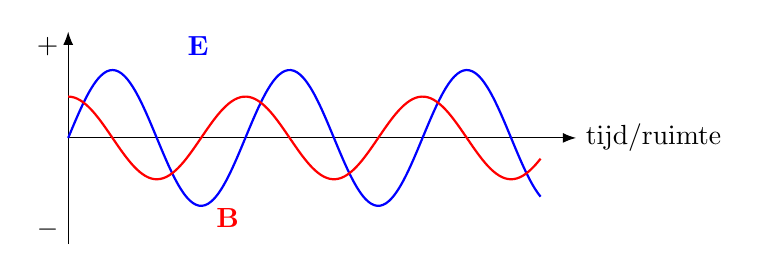
\begin{tikzpicture}[x=0.75cm,y=0.75cm,>=Latex]
  \draw[->] (0,0)--(8.6,0) node[right] {tijd/ruimte};
  \draw[->] (0,-1.8)--(0,1.8);
  \draw[blue,thick,domain=0:8,samples=160,smooth]
       plot(\x,{1.15*sin(120*\x)});
  \draw[red,thick,domain=0:8,samples=160,smooth]
       plot(\x,{0.7*cos(120*\x)});
  \node[blue] at (2.2,1.55) {$\mathbf{E}$};
  \node[red] at (2.7,-1.35) {$\mathbf{B}$};
  \node[left] at (0,1.55) {$+$};
  \node[left] at (0,-1.55) {$-$};
\end{tikzpicture}
\end{center}

\subsubsection*{Röntgenstraal}

\begin{center}
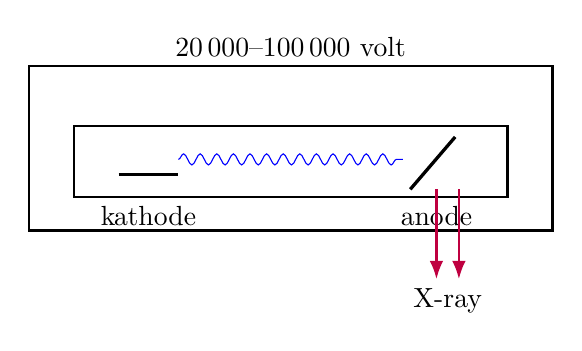
\begin{tikzpicture}[>=Latex,scale=0.95]
  \draw[thick] (0,0) rectangle (7,2.2);
  \draw[thick] (0.6,0.45) rectangle (6.4,1.4);
  \draw[very thick] (1.2,0.75)--(2.0,0.75);
  \node[below] at (1.6,0.45) {kathode};
  \draw[very thick] (5.1,0.55)--(5.7,1.25);
  \node[below] at (5.45,0.45) {anode};
  \draw[blue,decorate,decoration={snake,amplitude=2pt,segment length=6pt}]
       (2.0,0.95)--(5.0,0.95);
  \draw[purple,->,thick] (5.45,0.55)--(5.45,-0.65);
  \draw[purple,->,thick] (5.75,0.55)--(5.75,-0.65);
  \node[below] at (5.6,-0.65) {X-ray};
  \node[above,align=center] at (3.5,2.2)
       {$20\,000$--$100\,000$ volt};
\end{tikzpicture}
\end{center}

\subsection*{Rechter notitiepagina}

\begin{align*}
\text{fonon} &\longrightarrow \text{geluid},\\
             &\text{mechanische energie}.
\end{align*}

\begin{center}
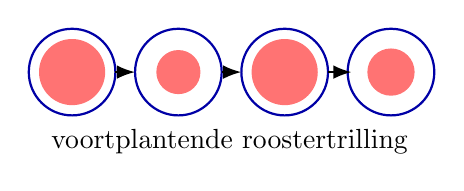
\begin{tikzpicture}[>=Latex]
  \foreach \x/\r in {0/0.42,1.35/0.28,2.7/0.42,4.05/0.3}
  {
    \draw[thick,blue!65!black] (\x,0) circle (0.55);
    \fill[red!55] (\x,0) circle (\r);
  }
  \draw[->,thick] (0.55,0)--(0.8,0);
  \draw[->,thick] (1.9,0)--(2.15,0);
  \draw[->,thick] (3.25,0)--(3.55,0);
  \node[below=0.6cm] at (2.0,0) {voortplantende roostertrilling};
\end{tikzpicture}
\end{center}

\literalnote{\centering Warmte $\Rightarrow$ trillende kern.}

\begin{center}
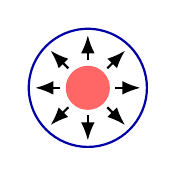
\begin{tikzpicture}[>=Latex]
  \draw[blue!65!black,thick] (0,0) circle (0.75);
  \fill[red!60] (0,0) circle (0.28);
  \foreach \a in {0,45,...,315}
    \draw[->,thick] ({0.35*cos(\a)},{0.35*sin(\a)})
      --({0.67*cos(\a)},{0.67*sin(\a)});
\end{tikzpicture}
\end{center}

\newpage
\section*{PDF-pagina 5 --- foto-elektrisch effect}

\subsection*{Linker notitiepagina}

\begin{center}
{\Large \textbf{Foto-elektrisch effect}}
\end{center}

\begin{center}
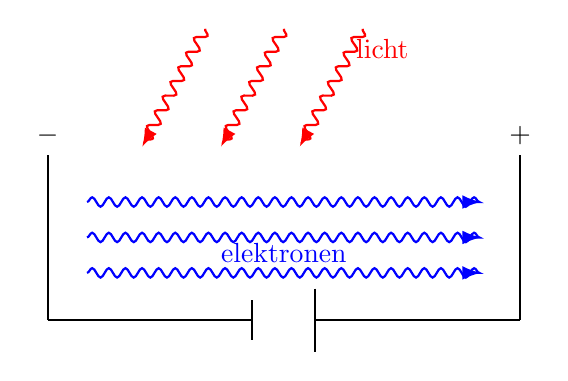
\begin{tikzpicture}[>=Latex,scale=1.0]
  % circuit and plates
  \draw[thick] (-3,-1.7)--(-3,0.4);
  \draw[thick] (3,-1.7)--(3,0.4);
  \draw[thick] (-3,-1.7)--(-0.4,-1.7);
  \draw[thick] (0.4,-1.7)--(3,-1.7);
  \draw[thick] (-0.4,-1.45)--(-0.4,-1.95);
  \draw[thick] (0.4,-1.3)--(0.4,-2.1);
  \node[above] at (-3,0.4) {$-$};
  \node[above] at (3,0.4) {$+$};

  % incident light
  \foreach \x in {-1.0,0,1.0}
    \draw[red,decorate,decoration={snake,amplitude=2pt,segment length=6pt},->,thick]
      (\x,2.0)--(\x-0.8,0.5);
  \node[red] at (1.25,1.75) {licht};

  % electrons
  \foreach \y in {-0.2,-0.65,-1.1}
    \draw[blue,decorate,decoration={snake,amplitude=1.7pt,segment length=6pt},->,thick]
      (-2.5,\y)--(2.5,\y);
  \node[blue] at (0,-0.85) {elektronen};
\end{tikzpicture}
\end{center}

\begin{align*}
E &= hf.
\end{align*}

\literalnote{\centering Hogere frequentie = meer elektronen los.}

De constante van Planck staat genoteerd als:

$$
h=6{,}62606957\cdot10^{-34}\ \mathrm{J/sec}.
$$

\noindent
De eenheid hierboven is letterlijk overgenomen uit de notitie.
De gebruikelijke SI-eenheid voor $h$ is $\mathrm{J\,s}$.

\subsection*{Rechter notitiepagina}

Genormaliseerde betekenis van de bovenste notatie:

\begin{align*}
1\,\mathrm{THz} &= 10^{12}\,\mathrm{Hz},\\
1\,\mathrm{nm}  &= 10^{-9}\,\mathrm{m}.
\end{align*}

\begin{center}
\small
\begin{tabular}{lrrrrrrr}
\toprule
 & infrarood & rood & oranje & geel & groen & blauw & violet\\
\midrule
$f$ ($\mathrm{THz}$)       & 380 & 460 & 510 & 525 & 590 & 620 & 750\\
$\lambda$ ($\mathrm{nm}$)  & 780 & 650 & 590 & 570 & 510 & 475 & 400\\
$E$ ($\mathrm{eV}$)        & 1.6 & 1.9 & 2.1 & 2.2 & 2.4 & 2.6 & 3.1\\
\bottomrule
\end{tabular}
\end{center}

\begin{center}
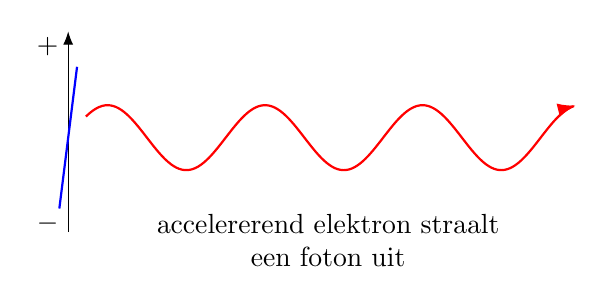
\begin{tikzpicture}[>=Latex,x=0.75cm,y=0.75cm]
  \draw[->] (0,-1.6)--(0,1.8);
  \node[left] at (0,1.55) {$+$};
  \node[left] at (0,-1.45) {$-$};
  \draw[blue,thick] (-0.15,-1.2)--(0.15,1.2);
  \draw[red,thick,domain=0.3:8.6,samples=180,smooth,->]
       plot(\x,{0.55*sin(135*\x)});
  \node[below=0.7cm,align=center] at (4.4,-0.2)
       {accelererend elektron straalt\\een foton uit};
\end{tikzpicture}
\end{center}

\end{document}
